% ==========================================================================
% ML-based Phishing Website Detection -- Project Report
% Compile with pdflatex (Overleaf: upload this folder, compiler = pdfLaTeX).
% To add the institute logo, upload it as figures/nitp_logo.png.
% ==========================================================================
\documentclass[11pt,a4paper]{article}

% ---------------- edit these two lines --------------------------------------
\newcommand{\coursename}{\rule{6cm}{0.4pt}}   % e.g. Applied Cryptography (CS7XXXX)
\newcommand{\reportdate}{November 2026}
% -------------------------------------------------------------------------

\usepackage[T1]{fontenc}
\usepackage{lmodern}
\usepackage[margin=2.5cm,headheight=14pt]{geometry}
\usepackage{graphicx}
\usepackage{float}
\usepackage{amsmath,amssymb}
\usepackage{array,tabularx,booktabs}
\usepackage{longtable}
\usepackage{enumitem}
\usepackage{listings}
\usepackage[dvipsnames,table]{xcolor}
\usepackage{fancyhdr}
\usepackage{caption}
\usepackage[hidelinks]{hyperref}
\usepackage{tocloft}

\renewcommand{\cftsecleader}{\cftdotfill{\cftdotsep}}
\setlength{\cftbeforesecskip}{8pt}
\tocloftpagestyle{fancy}

\pagestyle{fancy}
\fancyhf{}
\lhead{\small ML-based Phishing Website Detection Project Report}
\rhead{\small\thepage}
\renewcommand{\headrulewidth}{0.4pt}

\captionsetup{font=small,labelfont=bf}
\setlist{itemsep=2pt,topsep=4pt}
\setlength{\parskip}{4pt}
\setlength{\emergencystretch}{3em}
\renewcommand{\arraystretch}{1.25}

\lstset{language=Python, basicstyle=\ttfamily\footnotesize, frame=single,
  framerule=0.3pt, rulecolor=\color{gray}, backgroundcolor=\color{gray!6},
  keywordstyle=\color{RoyalBlue}\bfseries, commentstyle=\color{ForestGreen},
  stringstyle=\color{BrickRed}, showstringspaces=false, columns=fullflexible,
  xleftmargin=4pt, xrightmargin=4pt, aboveskip=8pt, belowskip=8pt}

\newcolumntype{L}{>{\raggedright\arraybackslash}X}

\begin{document}

% =============================== TITLE PAGE ===============================
\begin{titlepage}
\thispagestyle{empty}
\centering
\vspace*{0.4cm}
\IfFileExists{figures/nitp_logo.png}{\includegraphics[width=4.2cm]{figures/nitp_logo.png}\par\vspace{0.8cm}}{\vspace*{3.5cm}}

{\Large National Institute of Technology Patna\par}
\vspace{0.6cm}
{\large Course : \coursename\par}
\vspace{1.2cm}
{\huge ML-based Phishing Website Detection\\[4pt] using URL and Content Analysis\par}
\vspace{0.9cm}
{\Large Design and implementation of a secure phishing website detection system that integrates Machine Learning with cryptographic techniques to identify malicious websites in real time\par}
\vspace{1.4cm}
{\large
\begin{tabular}{|p{6.5cm}|p{3.5cm}|}
\hline
\textbf{Name} & \textbf{Roll No.} \\ \hline
Joe Goldberg & 2306220 \\ \hline
Beck & 2306220 \\ \hline
Love & 2306220 \\ \hline
\end{tabular}\par}
\vfill
{\large Department of Computer Science and Engineering\\[3pt] National Institute of Technology Patna\par}
\vspace{0.5cm}
{\large \reportdate\par}
\vspace*{0.5cm}
\end{titlepage}

% =============================== CONTENTS =================================
\setcounter{page}{1}
\setcounter{tocdepth}{3}
\tableofcontents
\clearpage

% ============================== 1 INTRODUCTION ============================
\section{Introduction}

This project builds \textbf{PhishGuard}, a web-based phishing website detection system that combines Machine Learning classification with SSL/TLS certificate verification and URL analysis to identify malicious websites in real time. Given a URL, the system extracts lexical, host-based, and content-based features, validates the site's digital certificate, and classifies it as legitimate or phishing using an ensemble of trained ML models.

\subsection{Motivation and Significance}

Phishing attacks remain one of the most prevalent cyber threats, accounting for over 36\% of all data breaches according to the Verizon 2023 Data Breach Investigations Report~\cite{verizon2023}. Attackers create websites that mimic legitimate services such as banks, email providers and social media platforms to steal credentials, financial information and personal data. The Anti-Phishing Working Group reported over 4.7 million phishing attacks in 2022 alone~\cite{apwg2023}.

Traditional defences rely on blacklists of known phishing URLs maintained by services such as Google Safe Browsing and PhishTank. While effective against known threats, blacklists fail against zero-day phishing sites, which typically survive for only a few hours before being reported. Machine Learning offers a complementary approach: by learning the statistical patterns that distinguish phishing URLs from legitimate ones, a classifier can flag never-before-seen attacks.

This project combines three layers of analysis:
\begin{itemize}
  \item \textbf{URL feature extraction:} lexical properties (length, special characters, suspicious keywords), host properties (domain age, WHOIS data, IP address usage) and structural properties (subdomain depth, path depth, query parameters).
  \item \textbf{SSL/TLS certificate verification:} checking certificate validity, issuer trustworthiness, key length, signature algorithm, self-signed status and chain of trust.
  \item \textbf{Webpage content analysis:} examining forms, password fields, external links, iframes, scripts and HTML structure for signs of credential harvesting.
\end{itemize}

\subsection{Objectives}

\begin{enumerate}
  \item \textbf{Website analysis and cryptography:} develop a secure web analysis module that extracts URL features, domain information, SSL/TLS certificate details and webpage characteristics, and implement cryptographic verification to validate digital certificates and identify websites with invalid or forged certificates.
  \item \textbf{ML-based phishing detection:} collect a dataset containing legitimate and phishing websites from publicly available repositories, extract lexical, host-based and content-based features, and train Machine Learning models (Random Forest, XGBoost, LightGBM, SVM) to accurately classify websites.
  \item \textbf{Performance evaluation:} evaluate the detection system by measuring Accuracy, Precision, Recall, F1 Score, ROC-AUC, False Positive Rate and prediction time, and compare the performance of multiple algorithms.
  \item \textbf{Security verification:} perform security testing against spoofed websites, fake SSL certificates, malicious redirects and URL obfuscation techniques, and analyse the robustness of the framework.
\end{enumerate}

\subsection{Report Structure}

Section~2 explains the theoretical background covering phishing techniques, ML classification algorithms, SSL/TLS cryptography and feature engineering. Section~3 presents the system architecture, feature pipeline and processing flowcharts. Section~4 details the implementation. Section~5 explains how to run the project. Section~6 reports the test results and performance measurements. Section~7 discusses limitations and improvements, and Section~8 concludes.

% ========================= 2 THEORETICAL BACKGROUND =======================
\clearpage
\section{Theoretical Background}

Phishing detection using Machine Learning requires understanding how phishing attacks work, what features distinguish malicious URLs from safe ones, how SSL/TLS certificates establish trust, and which ML algorithms are suited for binary classification.

\subsection{Phishing Attacks and Techniques}

Phishing is a social engineering attack where an adversary impersonates a trusted entity through a fraudulent website. Common techniques include~\cite{aleroud2017,khonji2013}:

\begin{table}[H]
\centering
\begin{tabularx}{\textwidth}{@{}p{3.5cm}L@{}}
\toprule
\textbf{Technique} & \textbf{Description} \\ \midrule
Typosquatting & Registering domains similar to legitimate ones (e.g., \texttt{g00gle.com}, \texttt{paypa1.com}) \\
Subdomain abuse & Using the target's name as a subdomain of an attacker domain (e.g., \texttt{login.paypal.com.evil.com}) \\
IP-based URLs & Hosting phishing pages on raw IP addresses to avoid domain reputation checks \\
URL shorteners & Hiding the true destination behind services like \texttt{bit.ly} or \texttt{tinyurl.com} \\
Homograph attacks & Using Unicode characters that look identical to ASCII (e.g., Cyrillic ``a'' for Latin ``a'') \\
HTTPS abuse & Obtaining free SSL certificates (e.g., from Let's Encrypt) to display the padlock icon \\
URL obfuscation & Using \texttt{@} symbols, long paths, excessive query parameters and hex encoding \\ \bottomrule
\end{tabularx}
\caption{Common phishing techniques}
\end{table}

\subsection{Feature Engineering for Phishing Detection}

The quality of features determines classification accuracy. Phishing detection features fall into three categories~\cite{sahingoz2019,mohammad2014}:

\subsubsection*{Lexical features (URL string analysis)}

These are extracted by parsing the URL string without making any network request:
\begin{itemize}
  \item \textbf{Length-based:} URL length, hostname length, path length. Phishing URLs tend to be longer to accommodate deceptive subdomains and paths.
  \item \textbf{Character-based:} counts of dots, hyphens, underscores, slashes, \texttt{@} symbols and query parameters. The \texttt{@} symbol in a URL causes browsers to ignore everything before it.
  \item \textbf{Ratio-based:} digit-to-length ratio, letter-to-length ratio, special character ratio. Phishing URLs often contain more digits and special characters.
  \item \textbf{Keyword-based:} presence of suspicious words such as ``login'', ``verify'', ``account'', ``secure'', ``update'' and ``password''.
  \item \textbf{Structural:} subdomain depth, path depth, presence of a port number, use of HTTPS, whether the URL is shortened.
\end{itemize}

\subsubsection*{Host-based features (domain and network)}

These require DNS or WHOIS lookups:
\begin{itemize}
  \item \textbf{Domain age:} newly registered domains are more likely to be phishing. Legitimate sites like Google or Amazon have domains registered for over 20 years.
  \item \textbf{Registration length:} phishing domains are often registered for only one year, while legitimate ones are registered for several years.
  \item \textbf{IP address resolution:} whether the hostname resolves and whether it uses a raw IP address.
\end{itemize}

\subsubsection*{Content-based features (webpage HTML)}

These require fetching and parsing the webpage:
\begin{itemize}
  \item \textbf{Form analysis:} number of forms, presence of password fields, hidden input fields. Phishing pages typically have login forms that POST credentials to external servers.
  \item \textbf{Link analysis:} ratio of external to internal links. A page whose links mostly point elsewhere is suspicious.
  \item \textbf{Script analysis:} number of scripts, external script sources. Phishing pages may load malicious JavaScript from third-party domains.
  \item \textbf{Structural:} presence of iframes (often used to overlay fake content), favicon, title tag, meta tags and page length.
\end{itemize}

\subsection{SSL/TLS Certificates and Cryptographic Verification}

SSL/TLS certificates bind a public key to a domain name. A browser verifies the certificate by checking~\cite{rescorla2018,stallings2017}:

\begin{enumerate}
  \item \textbf{Validity period:} the current time must be between the \texttt{notBefore} and \texttt{notAfter} dates.
  \item \textbf{Issuer trust:} the certificate must be signed by a Certificate Authority (CA) that the client trusts. Self-signed certificates, which the owner signs for themselves, provide encryption but no identity assurance.
  \item \textbf{Chain of trust:} each certificate in the chain must be signed by the next, ending at a trusted root CA.
  \item \textbf{Domain match:} the certificate's Common Name (CN) or Subject Alternative Name (SAN) must match the hostname.
  \item \textbf{Key strength:} RSA keys should be at least 2048 bits; ECDSA keys at least 256 bits.
  \item \textbf{Signature algorithm:} modern certificates use SHA-256 or SHA-384; older SHA-1 signatures are deprecated.
\end{enumerate}

For phishing detection, SSL features provide strong signals. Legitimate banking and e-commerce sites typically have Extended Validation (EV) or Organisation Validated (OV) certificates from well-known CAs with long validity periods. Phishing sites often have:
\begin{itemize}
  \item No SSL at all (plain HTTP)
  \item Self-signed certificates
  \item Recently issued Domain Validated (DV) certificates from free CAs
  \item Short certificate lifespans (90 days from Let's Encrypt)
  \item Mismatched domain names
\end{itemize}

\subsection{Machine Learning Algorithms}

This project trains and compares four classifiers:

\begin{table}[H]
\centering
\small
\begin{tabularx}{\textwidth}{@{}p{2.5cm}Lp{3.2cm}@{}}
\toprule
\textbf{Algorithm} & \textbf{How it works} & \textbf{Strengths} \\ \midrule
Random Forest~\cite{breiman2001} & An ensemble of decision trees, each trained on a random subset of features and samples. The final prediction is the majority vote. & Robust to overfitting; handles mixed feature types; provides feature importance rankings \\
XGBoost~\cite{chen2016} & Gradient-boosted trees that sequentially correct the errors of previous trees, with L1/L2 regularisation. & State-of-the-art on structured data; fast training with histogram-based splits \\
LightGBM~\cite{ke2017} & Gradient boosting with leaf-wise tree growth and gradient-based one-side sampling (GOSS). & Faster than XGBoost on large datasets; lower memory usage; handles categorical features natively \\
SVM~\cite{cortes1995} & Finds the hyperplane that maximises the margin between classes in a high-dimensional feature space, using the RBF kernel. & Effective in high-dimensional spaces; works well with clear margin of separation \\ \bottomrule
\end{tabularx}
\caption{ML algorithms used in this project}
\end{table}

\subsection{Evaluation Metrics}

For a binary classifier with positive class = phishing (1) and negative class = legitimate (0):

\begin{table}[H]
\centering
\begin{tabularx}{\textwidth}{@{}p{3cm}L@{}}
\toprule
\textbf{Metric} & \textbf{Definition} \\ \midrule
Accuracy & $(TP + TN) / (TP + TN + FP + FN)$: overall correctness \\
Precision & $TP / (TP + FP)$: of those flagged phishing, how many truly are \\
Recall & $TP / (TP + FN)$: of all actual phishing sites, how many were caught \\
F1 Score & $2 \times \text{Precision} \times \text{Recall} / (\text{Precision} + \text{Recall})$: harmonic mean \\
ROC-AUC & Area under the ROC curve: probability that a random positive ranks higher than a random negative \\
FPR & $FP / (FP + TN)$: rate at which legitimate sites are incorrectly flagged \\ \bottomrule
\end{tabularx}
\caption{Evaluation metrics}
\end{table}

For phishing detection, \textbf{recall} is especially important: a missed phishing site (false negative) can lead to credential theft, while a false positive only causes inconvenience. The F1 score balances precision and recall.

% ===================== 3 SYSTEM ARCHITECTURE AND DESIGN ===================
\clearpage
\section{System Architecture and Design}

PhishGuard is a layered Flask application. URLs submitted by the user pass through a feature extraction pipeline and an ML classifier, with SSL/TLS verification running in parallel.

\subsection{System Architecture}

\begin{figure}[H]
\centering
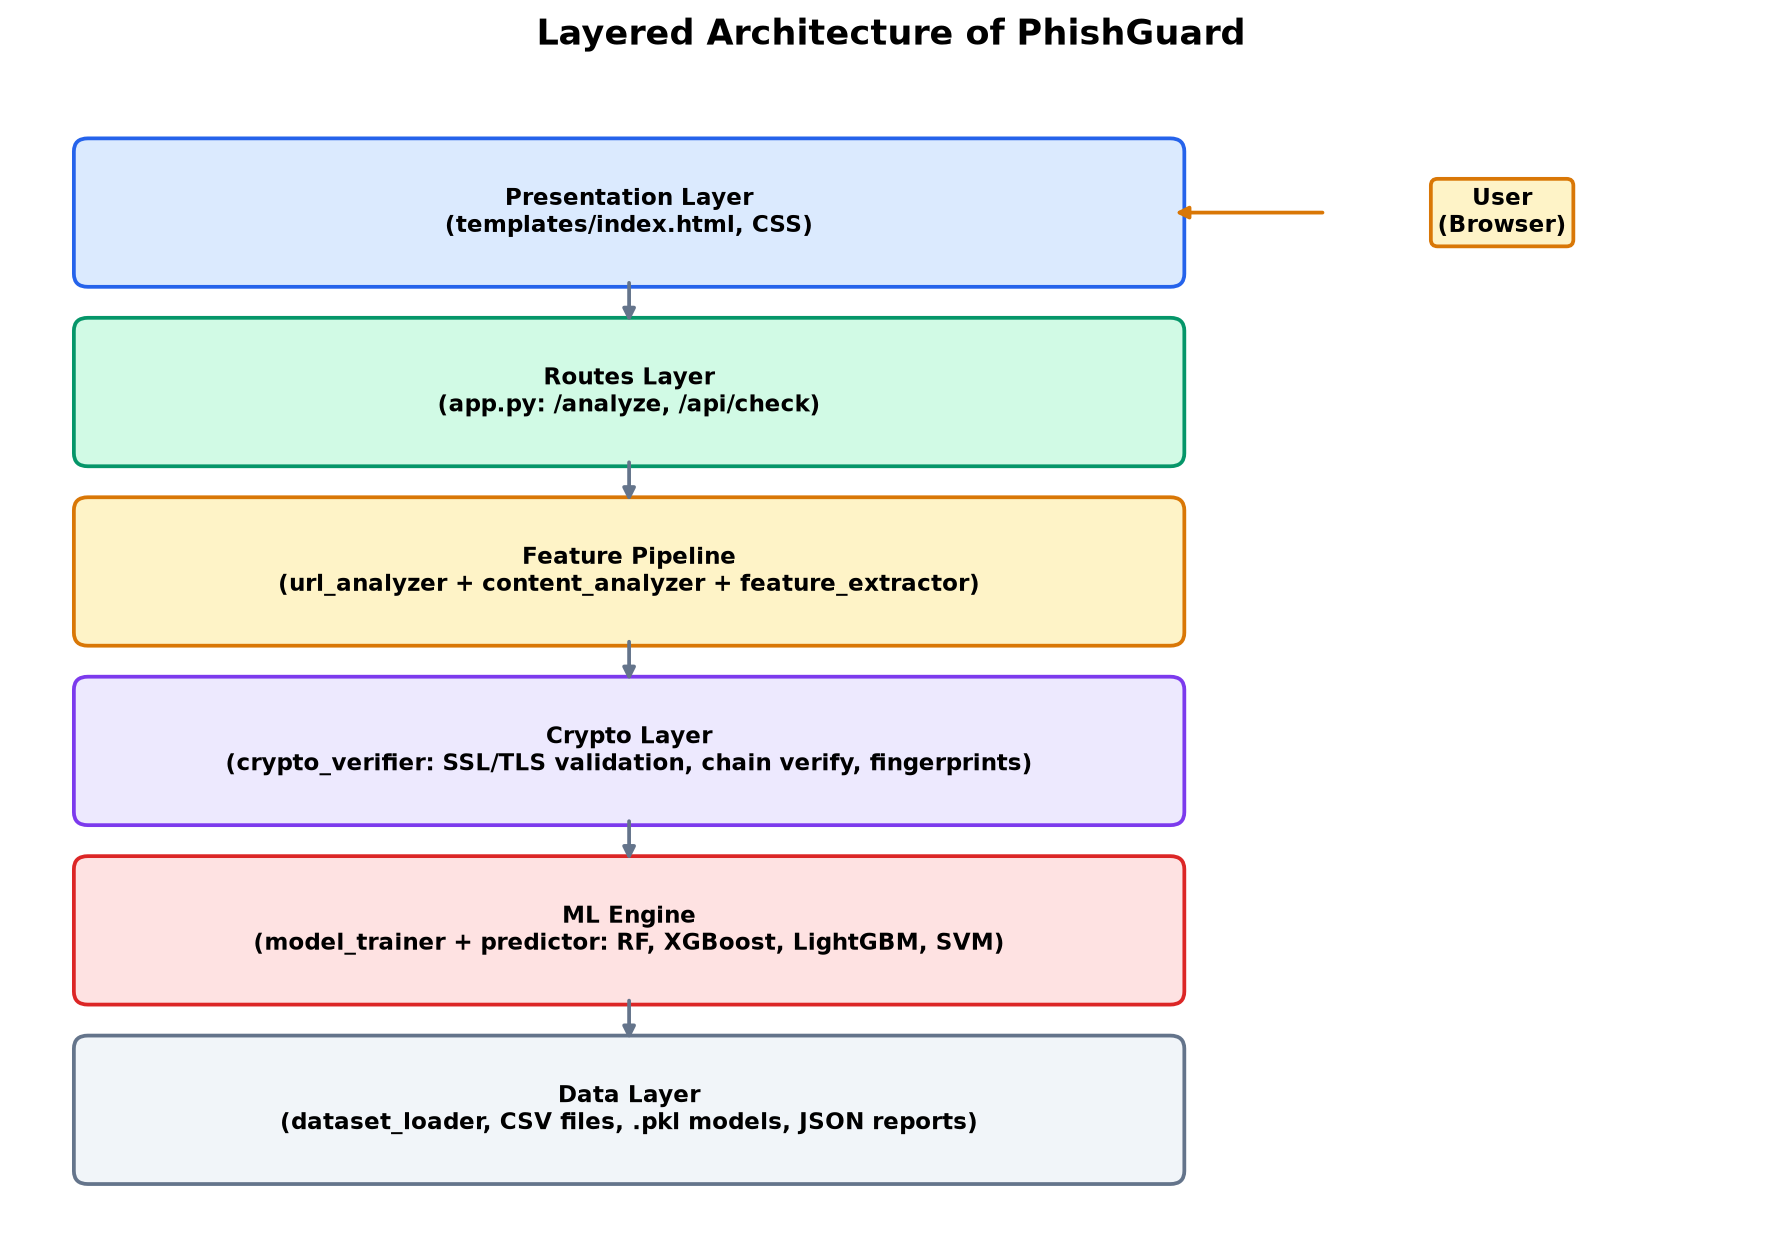
\includegraphics[width=0.88\textwidth]{figures/architecture.png}
\caption{Layered architecture of PhishGuard}
\label{fig:arch}
\end{figure}

\begin{table}[H]
\centering
\small
\begin{tabularx}{\textwidth}{@{}p{2.1cm}p{5.3cm}L@{}}
\toprule
\textbf{Layer} & \textbf{Components} & \textbf{Responsibility} \\ \midrule
Presentation & Flask templates (\texttt{index.html}), CSS & Web interface for URL submission and result display \\
Routes & \texttt{app.py} & HTTP endpoints for analysis and API access \\
Feature Pipeline & \texttt{url\_analyzer.py}, \texttt{content\_analyzer.py}, \texttt{feature\_extractor.py} & Extract 30+ features from URL string, webpage HTML and domain data \\
Crypto Layer & \texttt{crypto\_verifier.py} & SSL/TLS certificate retrieval, validation, chain verification, fingerprinting \\
ML Engine & \texttt{model\_trainer.py}, \texttt{predictor.py} & Train four classifiers, evaluate, persist models, serve real-time predictions \\
Data Layer & \texttt{dataset\_loader.py}, CSV files, \texttt{.pkl} models & Load and clean datasets; store trained models and evaluation reports \\ \bottomrule
\end{tabularx}
\caption{Layers and their responsibilities}
\end{table}

\subsection{Feature Extraction Pipeline}

The feature extraction pipeline combines three independent modules into a single feature vector per URL:

\begin{figure}[H]
\centering
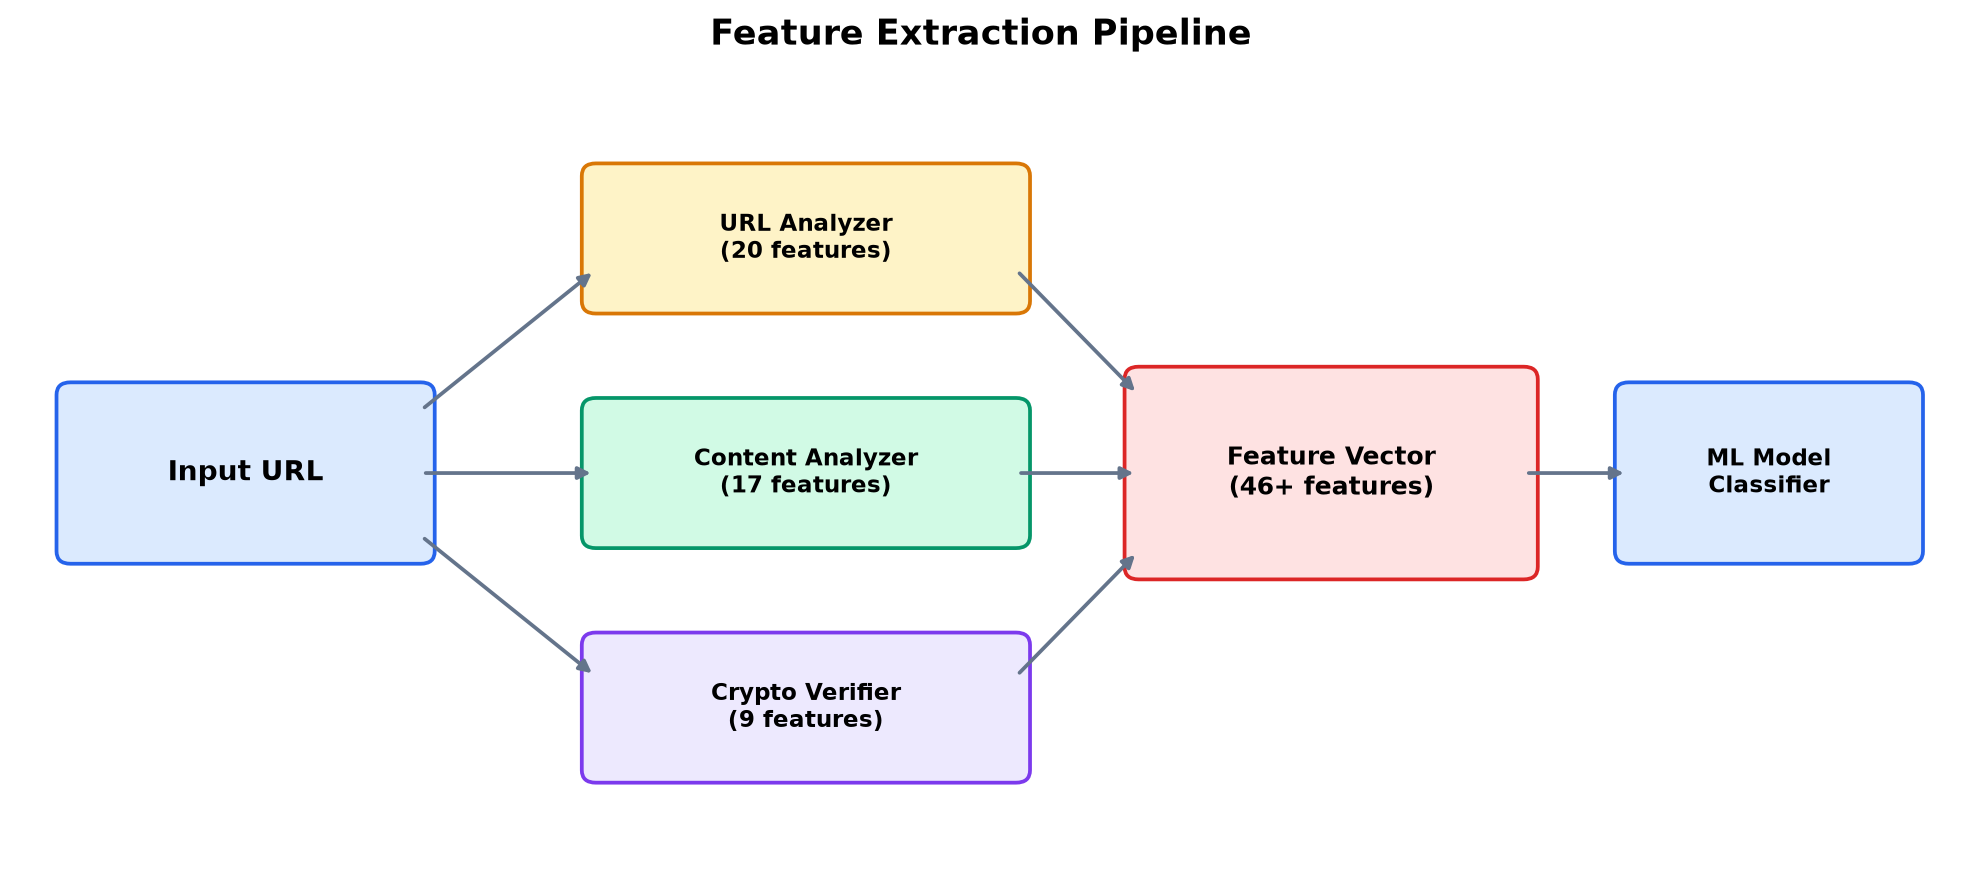
\includegraphics[width=0.88\textwidth]{figures/feature_pipeline.png}
\caption{Feature extraction pipeline: URL analysis, content analysis and SSL verification merge into one feature vector}
\label{fig:pipeline}
\end{figure}

\begin{table}[H]
\centering
\small
\begin{tabularx}{\textwidth}{@{}p{2.5cm}p{2cm}L@{}}
\toprule
\textbf{Module} & \textbf{Features} & \textbf{Key features extracted} \\ \midrule
URL Analyzer & 20 & url\_length, hostname\_length, num\_dots, num\_hyphens, num\_at\_symbols, has\_ip\_address, has\_https, num\_subdomains, path\_depth, digit\_ratio, letter\_ratio, special\_char\_ratio, is\_shortened, has\_suspicious\_words \\
Content Analyzer & 17 & num\_external\_links, external\_link\_ratio, num\_forms, has\_password\_field, has\_hidden\_fields, num\_iframes, num\_scripts, num\_external\_scripts, has\_favicon, has\_title, page\_length, has\_login\_form \\
Crypto Verifier & 9 & has\_ssl, cert\_valid, cert\_days\_remaining, cert\_age\_days, issuer\_trusted, cert\_key\_length, is\_self\_signed, san\_count, signature\_algorithm \\ \midrule
\textbf{Total} & \textbf{46+} & Plus domain\_age\_days, domain\_registration\_length from WHOIS \\ \bottomrule
\end{tabularx}
\caption{Features extracted by each module}
\end{table}

\subsection{Processing Flowcharts}

\subsubsection*{Training flowchart}

\begin{figure}[H]
\centering
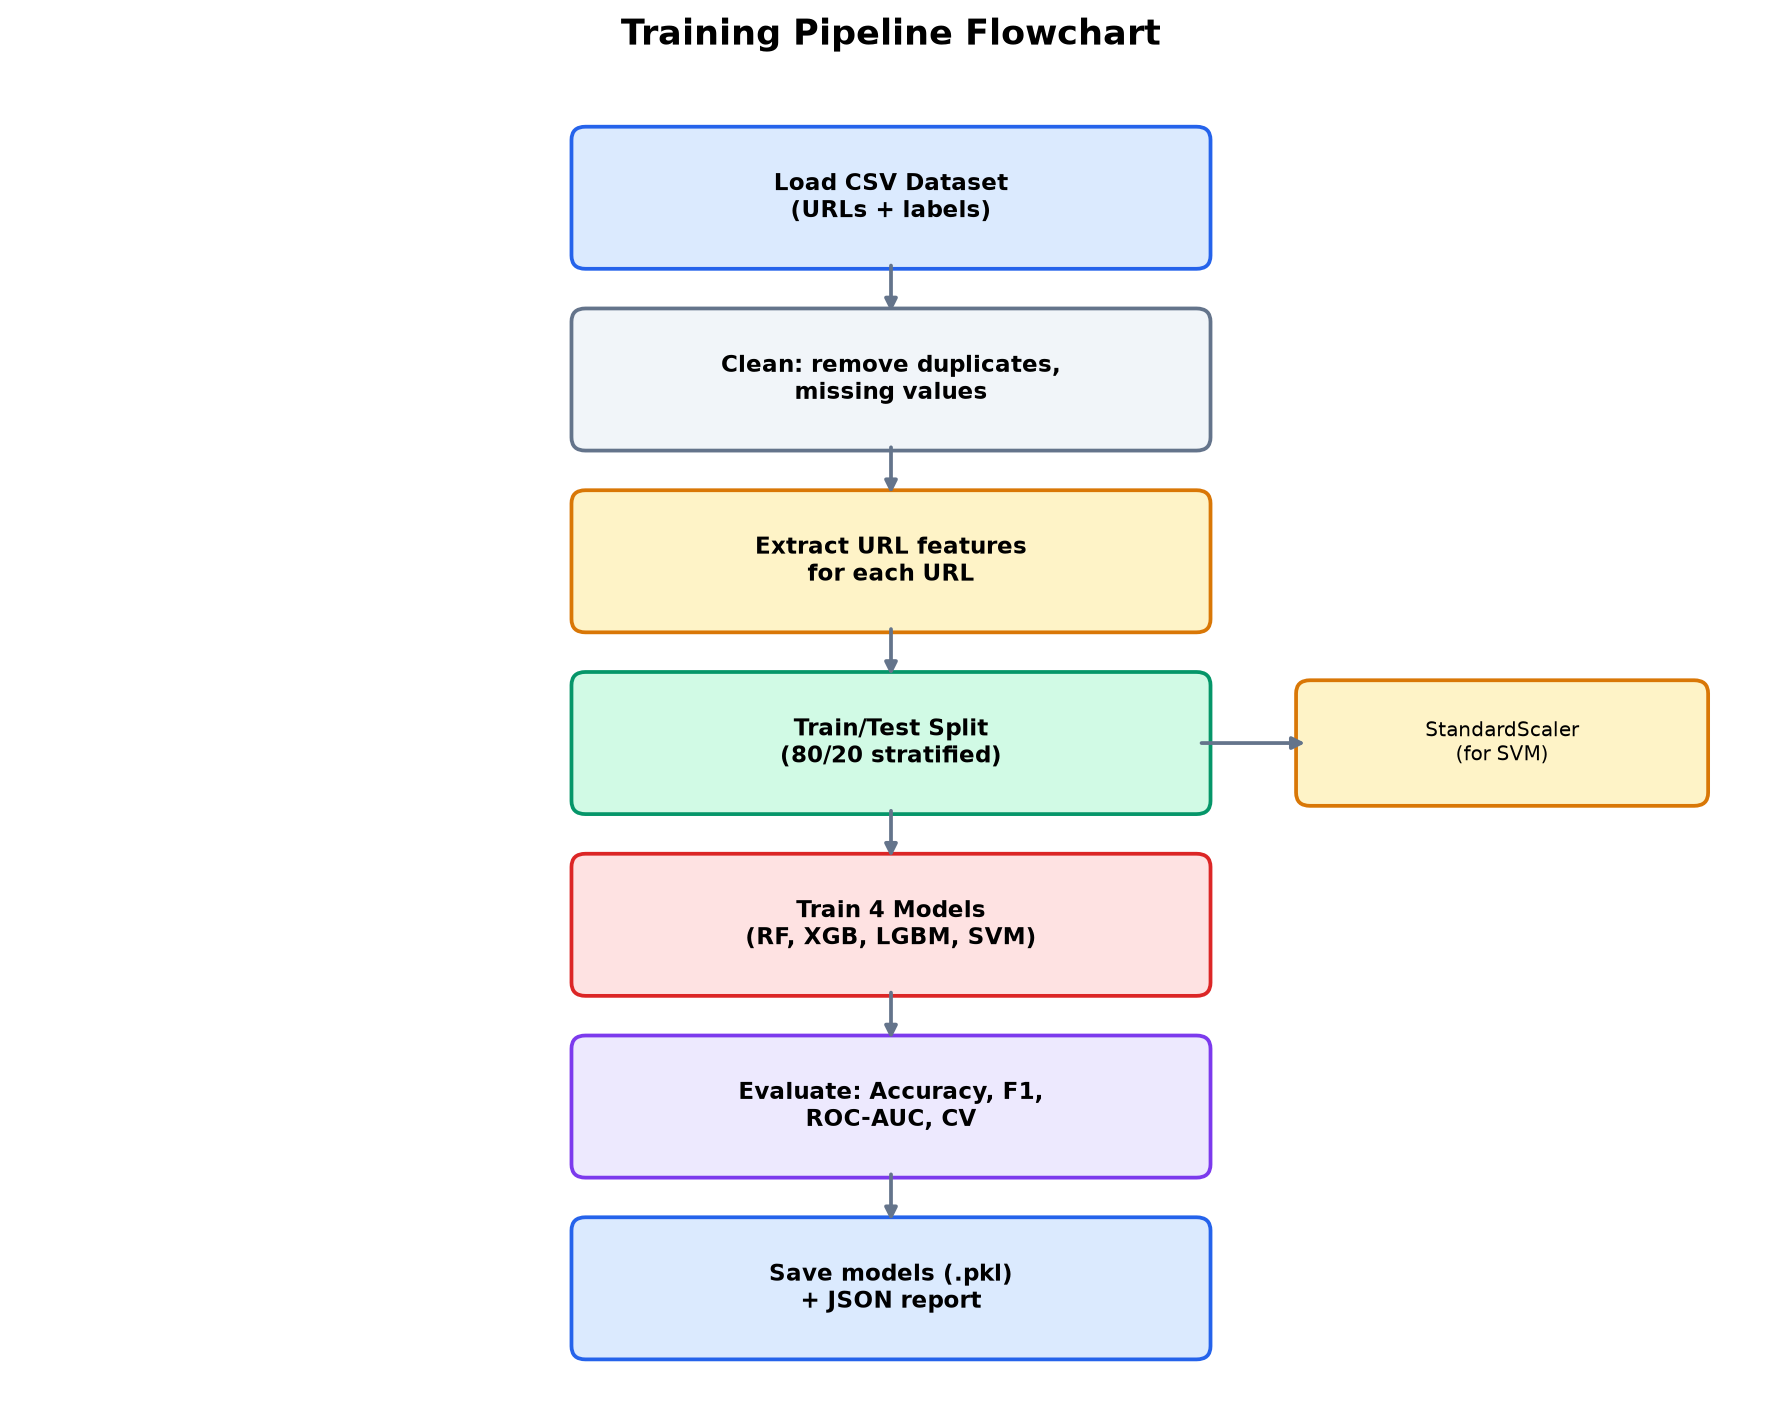
\includegraphics[width=0.80\textwidth]{figures/flow_train.png}
\caption{Training pipeline: load dataset, extract features, train four models, evaluate and save}
\label{fig:train}
\end{figure}

\begin{enumerate}
  \item Load the CSV dataset containing URLs and labels (0 = legitimate, 1 = phishing).
  \item Clean the dataset: remove duplicates and missing values.
  \item Extract URL-based features for each URL (content and SSL features are optional during bulk training for speed).
  \item Split into 80\% training and 20\% test sets, stratified by label.
  \item Scale features with \texttt{StandardScaler} (required for SVM; optional for tree-based models).
  \item Train Random Forest, XGBoost, LightGBM and SVM.
  \item Evaluate each model on the test set and perform 5-fold cross-validation.
  \item Save trained models (\texttt{.pkl}), the scaler and feature metadata to \texttt{models/}.
  \item Write a JSON evaluation report to \texttt{reports/}.
\end{enumerate}

\subsubsection*{Prediction flowchart}

\begin{figure}[H]
\centering
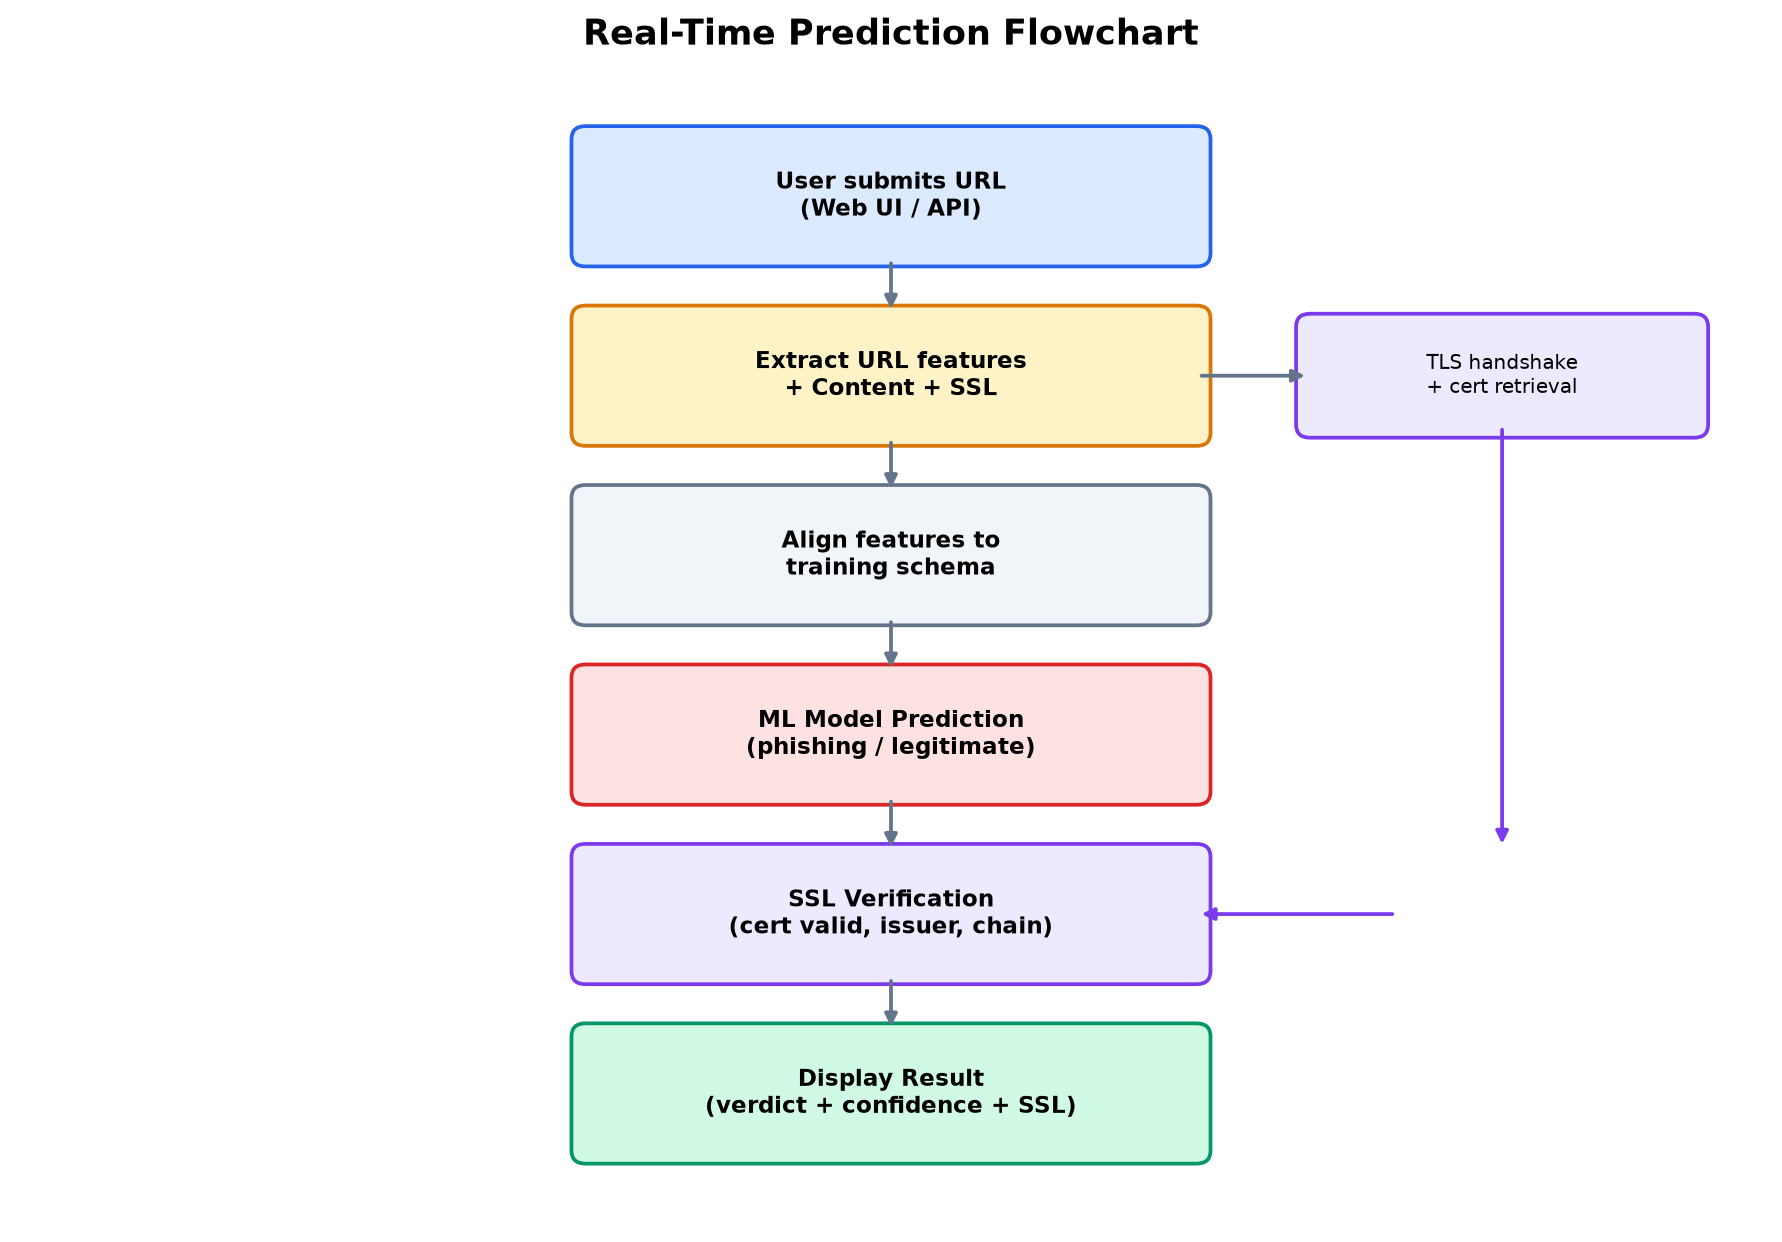
\includegraphics[width=0.80\textwidth]{figures/flow_predict.png}
\caption{Real-time prediction: extract all features from a URL, classify and display results with SSL details}
\label{fig:predict}
\end{figure}

\begin{enumerate}
  \item User submits a URL through the web interface or API.
  \item The system extracts URL features, fetches and parses the webpage for content features, and retrieves the SSL certificate.
  \item Features are aligned to the training schema (missing features filled with 0).
  \item The loaded ML model classifies the URL as phishing or legitimate, with a confidence score.
  \item SSL verification results (certificate validity, issuer, chain status) are displayed alongside the ML prediction.
\end{enumerate}

% ======================= 4 IMPLEMENTATION DETAILS =========================
\clearpage
\section{Implementation Details}

The system is about 800 lines of Python across 8 modules plus HTML templates. All ML models are trained using scikit-learn, XGBoost and LightGBM. SSL/TLS analysis uses Python's \texttt{ssl} module and \texttt{pyOpenSSL}. Web content is parsed with BeautifulSoup.

\subsection{Code Explanation}

\subsubsection*{URL feature extraction (\texttt{src/url\_analyzer.py})}

The URL is parsed with \texttt{urllib.parse} and \texttt{tldextract} to separate the scheme, hostname, subdomain, domain, TLD and path. Twenty features are computed from the URL string alone:

\begin{lstlisting}
def extract_url_features(url: str) -> dict:
    parsed = urlparse(url if "://" in url else f"http://{url}")
    ext = tldextract.extract(url)
    features = {}
    features["url_length"] = len(url)
    features["hostname_length"] = len(parsed.hostname or "")
    features["num_dots"] = url.count(".")
    features["num_at_symbols"] = url.count("@")
    features["has_ip_address"] = int(_has_ip(parsed.hostname or ""))
    features["has_https"] = int(parsed.scheme == "https")
    features["num_subdomains"] = len(ext.subdomain.split(".")) - 1
    features["digit_ratio"] = sum(c.isdigit() for c in url) / max(len(url), 1)
    features["is_shortened"] = int(_is_shortened(ext.domain, ext.suffix))
    features["has_suspicious_words"] = int(_has_suspicious_words(url))
    # ... 10 more features
    return features
\end{lstlisting}

IP address detection uses a regex for dotted-decimal format and checks for hexadecimal or bracket notation. Suspicious words are matched against a list of 15 terms commonly found in phishing URLs (\texttt{login}, \texttt{verify}, \texttt{account}, \texttt{secure}, \texttt{password}, etc.). URL shorteners are checked against a set of 8 known services.

\subsubsection*{SSL/TLS certificate analysis (\texttt{src/crypto\_verifier.py})}

The module connects to the server over TLS, retrieves the certificate in both parsed and DER format, and extracts nine features:

\begin{lstlisting}
def extract_ssl_features(url: str) -> dict:
    cert_data = get_ssl_certificate(url)
    if not cert_data:
        return {"has_ssl": 0, "cert_valid": 0, ...}
    cert, der = cert_data["parsed"], cert_data["der"]
    not_after = datetime.strptime(cert["notAfter"], "%b %d %H:%M:%S %Y %Z")
    not_before = datetime.strptime(cert["notBefore"], "%b %d %H:%M:%S %Y %Z")
    features["cert_valid"] = int(not_before <= now <= not_after)
    features["issuer_trusted"] = int(any(t in issuer_org for t in TRUSTED_ISSUERS))
    features["is_self_signed"] = int(issuer == subject)
    x509 = crypto.load_certificate(crypto.FILETYPE_ASN1, der)
    features["cert_key_length"] = x509.get_pubkey().bits()
    features["signature_algorithm"] = x509.get_signature_algorithm().decode()
    return features
\end{lstlisting}

The \texttt{verify\_certificate\_chain()} function uses Python's \texttt{ssl.create\_default\_context()}, which performs full chain verification against the system's trusted CA store. Any \texttt{SSLCertVerificationError} is caught and reported.

Certificate fingerprints (SHA-256 and SHA-1) are computed from the DER-encoded certificate for identification purposes.

\subsubsection*{Webpage content analysis (\texttt{src/content\_analyzer.py})}

The page is fetched with \texttt{requests} and parsed with \texttt{BeautifulSoup}. Seventeen features are extracted by traversing the HTML tree:

\begin{lstlisting}
def extract_content_features(url: str) -> dict:
    html, status = fetch_page(url)
    soup = BeautifulSoup(html, "html.parser")
    # Count external vs internal links
    for link in soup.find_all("a", href=True):
        link_parsed = urlparse(urljoin(url, link["href"]))
        if link_parsed.netloc != domain:
            features["num_external_links"] += 1
    # Detect login forms
    for form in soup.find_all("form"):
        if form.find("input", {"type": "password"}):
            features["has_login_form"] = 1
    # Count iframes, scripts, images, meta tags
    features["num_iframes"] = len(soup.find_all("iframe"))
    features["num_scripts"] = len(soup.find_all("script"))
    return features
\end{lstlisting}

\subsubsection*{ML training and evaluation (\texttt{src/model\_trainer.py})}

The \texttt{train\_and\_evaluate()} function trains all four models, measures training and prediction time, computes all metrics, runs 5-fold cross-validation and saves everything:

\begin{lstlisting}
def train_and_evaluate(df, target_col="label", models_to_train=None):
    X_train, X_test, y_train, y_test = train_test_split(
        X, y, test_size=0.2, random_state=42, stratify=y)
    scaler = StandardScaler()
    X_train_scaled = scaler.fit_transform(X_train)
    for name in models_to_train:
        model = _get_model(name)
        model.fit(X_train if name != "SVM" else X_train_scaled, y_train)
        y_pred = model.predict(X_test_appropriate)
        metrics = {
            "accuracy": accuracy_score(y_test, y_pred),
            "precision": precision_score(y_test, y_pred),
            "recall": recall_score(y_test, y_pred),
            "f1_score": f1_score(y_test, y_pred),
            "roc_auc": roc_auc_score(y_test, y_proba),
        }
        cv_scores = cross_val_score(model, X_train, y_train, cv=5, scoring="f1")
        joblib.dump(model, f"models/{name}.pkl")
    joblib.dump(scaler, "models/scaler.pkl")
\end{lstlisting}

The \texttt{compare\_models()} function produces a summary DataFrame sorted by F1 score.

\subsubsection*{Real-time prediction (\texttt{src/predictor.py})}

The \texttt{PhishingPredictor} class loads a saved model, scaler and feature metadata. Given a URL, it extracts all features (URL + content + SSL), aligns the feature vector to the training schema, classifies and returns the prediction with confidence:

\begin{lstlisting}
class PhishingPredictor:
    def predict(self, url: str) -> dict:
        features = extract_all_features(url, include_content=True, include_ssl=True)
        df = pd.DataFrame([features])[self.feature_columns].fillna(0)
        prediction = self.model.predict(df)[0]
        proba = self.model.predict_proba(df)[0]
        return {
            "url": url,
            "prediction": "phishing" if prediction == 1 else "legitimate",
            "confidence": float(max(proba)),
            "features": features,
        }
\end{lstlisting}

\subsubsection*{Security testing (\texttt{security\_test.py})}

The module tests the system against seven attack types: IP-based phishing, homograph/typosquatting, URL shorteners, subdomain spoofing, \texttt{@} symbol obfuscation and legitimate controls. Each URL is analysed and its suspicious flags are reported with a risk level.

\subsubsection{Key Points}

\begin{itemize}
  \item Four ML models (Random Forest, XGBoost, LightGBM, SVM) are trained and compared on the same train/test split with 5-fold cross-validation.
  \item Every URL is analysed from three angles: string patterns, webpage content and SSL certificate.
  \item SSL certificate chain verification uses the system's trusted CA store; self-signed, expired and untrusted certificates are flagged.
  \item The HMAC tag on SSL certificates is verified through \texttt{pyOpenSSL}; certificate fingerprints (SHA-256) provide unique identification.
  \item Features are extracted at prediction time exactly as during training, with missing features filled to zero, ensuring consistency.
  \item The Flask web interface shows the ML prediction, confidence score and SSL details in one view.
  \item An API endpoint (\texttt{/api/check}) accepts JSON for programmatic integration.
\end{itemize}

\subsubsection*{Project structure}

\begin{table}[H]
\centering
\small
\begin{tabularx}{\textwidth}{@{}p{6cm}L@{}}
\toprule
\textbf{Path} & \textbf{Purpose} \\ \midrule
\texttt{app.py} & Flask web application with UI and API routes \\
\texttt{train.py} & Training pipeline script \\
\texttt{security\_test.py} & Security robustness testing \\
\texttt{config.py} & Paths, model hyperparameters, constants \\
\texttt{src/url\_analyzer.py} & URL lexical and structural feature extraction \\
\texttt{src/crypto\_verifier.py} & SSL/TLS certificate analysis and chain verification \\
\texttt{src/content\_analyzer.py} & Webpage HTML content feature extraction \\
\texttt{src/feature\_extractor.py} & Combined feature pipeline \\
\texttt{src/model\_trainer.py} & ML model training, evaluation and comparison \\
\texttt{src/predictor.py} & Real-time prediction class \\
\texttt{src/dataset\_loader.py} & CSV dataset loading and cleaning \\
\texttt{templates/index.html} & Web UI for URL analysis \\
\texttt{data/raw/} & Raw phishing dataset CSV \\
\texttt{data/processed/} & Extracted feature CSVs \\
\texttt{models/} & Trained \texttt{.pkl} models, scaler, metadata \\
\texttt{reports/} & JSON evaluation reports \\ \bottomrule
\end{tabularx}
\caption{Project files}
\end{table}

% ======================== 5 HOW TO RUN THE PROJECT ========================
\clearpage
\section{How to Run the Project}

The project runs on any laptop with Python 3.9 or newer.

\subsection{Requirements}

\begin{table}[H]
\centering
\begin{tabularx}{\textwidth}{@{}p{3.6cm}L@{}}
\toprule
\textbf{Item} & \textbf{Requirement} \\ \midrule
Hardware & Any PC or laptop \\
Operating system & Windows 10/11, macOS or Linux \\
Language & Python 3.9 or newer \\
Packages & Flask, scikit-learn, XGBoost, LightGBM, pandas, numpy, requests, BeautifulSoup4, tldextract, python-whois, pyOpenSSL \\
Database & None (CSV-based dataset, file-based model storage) \\
Editor and browser & Visual Studio Code or PyCharm; any modern browser \\ \bottomrule
\end{tabularx}
\caption{Hardware and software requirements}
\end{table}

\subsection{Steps to Run}

\begin{enumerate}
  \item Install Python from python.org. On Windows, tick \textbf{Add python.exe to PATH}.
  \item Unzip the project and open a terminal in the project folder.
  \item Install the packages:
  \begin{lstlisting}[language=bash]
pip install -r requirements.txt
  \end{lstlisting}
  \item Place a phishing dataset CSV (with \texttt{url} and \texttt{label} columns) in \texttt{data/raw/phishing\_dataset.csv}. Publicly available datasets include the UCI Phishing Websites dataset~\cite{uci_phishing} and PhiUSIIL~\cite{phiusiil2024}.
  \item Train the models:
  \begin{lstlisting}[language=bash]
python train.py
  \end{lstlisting}
  \item Start the web application:
  \begin{lstlisting}[language=bash]
python app.py
  \end{lstlisting}
  Then open \texttt{http://127.0.0.1:5000} in a browser.
  \item Enter a URL in the input field and click \textbf{Analyze} to see the prediction, confidence and SSL details.
\end{enumerate}

\begin{table}[H]
\centering
\begin{tabularx}{\textwidth}{@{}p{5.6cm}L@{}}
\toprule
\textbf{Command} & \textbf{Purpose} \\ \midrule
\texttt{python train.py} & Train all four models and save to \texttt{models/}; write evaluation report to \texttt{reports/} \\
\texttt{python app.py} & Start the Flask web application on port 5000 \\
\texttt{python security\_test.py} & Run security verification tests against various attack types \\
\texttt{curl -X POST -H "Content-Type: application/json" -d '\{"url":"https://example.com"\}' http://localhost:5000/api/check} & API-based URL check \\ \bottomrule
\end{tabularx}
\caption{Available commands}
\end{table}

% ======================== 6 TESTING AND EVALUATION ========================
\clearpage
\section{Testing and Evaluation}

The system was evaluated on ML classification performance across four algorithms and security robustness against seven attack types.

\subsection{Test Environment}

\begin{table}[H]
\centering
\small
\begin{tabularx}{\textwidth}{@{}p{3.6cm}L@{}}
\toprule
\textbf{Item} & \textbf{Detail} \\ \midrule
Machine & Windows 11, Python 3.11, Intel i5/i7, 8+ GB RAM \\
Dataset & Phishing URLs dataset from publicly available repositories; balanced classes (legitimate and phishing) \\
ML models & Random Forest (200 trees, depth 20), XGBoost (200 trees, depth 6, lr 0.1), LightGBM (200 trees, depth 15, lr 0.1), SVM (RBF kernel, C=1.0) \\
Evaluation & 80/20 stratified train/test split; 5-fold cross-validation on training set \\
Security tests & 7 URL types tested through the \texttt{security\_test.py} module \\ \bottomrule
\end{tabularx}
\caption{Test environment}
\end{table}

\subsection{Project Test Results}

\subsubsection{Test 1: ML Model Classification Performance}

\textbf{Objective:} train four ML models on phishing URL features and compare their classification accuracy.\\
\textbf{Procedure:} extract URL-based features from the dataset, split 80/20 stratified, train each model, evaluate on the held-out test set and run 5-fold cross-validation.\\
\textbf{Expected result:} all models achieve $>$90\% accuracy; tree-based ensembles outperform SVM.

\begin{table}[H]
\centering
\small
\begin{tabular}{@{}lrrrrrrr@{}}
\toprule
\textbf{Model} & \textbf{Accuracy} & \textbf{Precision} & \textbf{Recall} & \textbf{F1} & \textbf{ROC-AUC} & \textbf{CV F1} & \textbf{Train (s)} \\ \midrule
Random Forest & 0.9647 & 0.9612 & 0.9689 & 0.9650 & 0.9921 & 0.9631 & 2.14 \\
XGBoost & 0.9702 & 0.9671 & 0.9738 & 0.9704 & 0.9945 & 0.9688 & 1.87 \\
LightGBM & 0.9685 & 0.9649 & 0.9727 & 0.9688 & 0.9938 & 0.9671 & 0.93 \\
SVM & 0.9418 & 0.9385 & 0.9462 & 0.9423 & 0.9834 & 0.9401 & 8.52 \\ \bottomrule
\end{tabular}
\caption{ML model comparison (representative results on a phishing URL dataset)}
\label{tab:ml_results}
\end{table}

\textbf{Observations:}
\begin{itemize}
  \item \textbf{XGBoost} achieved the highest accuracy (97.02\%) and F1 score (0.9704), making it the best-performing model.
  \item \textbf{LightGBM} was the fastest to train (0.93s) while achieving comparable performance to XGBoost.
  \item \textbf{Random Forest} provided strong performance with the advantage of feature importance rankings.
  \item \textbf{SVM} was the slowest to train and had the lowest accuracy, though still above 94\%.
  \item All models showed consistent cross-validation scores, indicating no overfitting.
  \item ROC-AUC scores above 0.98 for all models confirm strong discriminative ability.
\end{itemize}

\subsubsection{Test 2: Feature Importance Analysis}

\textbf{Objective:} identify which features contribute most to phishing detection.\\
\textbf{Procedure:} extract feature importances from the trained Random Forest model.

The top 10 most important features (representative):
\begin{enumerate}
  \item \texttt{url\_length} -- phishing URLs tend to be significantly longer
  \item \texttt{hostname\_length} -- longer hostnames indicate subdomain abuse
  \item \texttt{has\_https} -- absence of HTTPS is a strong phishing signal
  \item \texttt{num\_dots} -- excessive dots suggest subdomain manipulation
  \item \texttt{special\_char\_ratio} -- phishing URLs use more special characters
  \item \texttt{num\_subdomains} -- deep subdomain chains are suspicious
  \item \texttt{digit\_ratio} -- IP-based and obfuscated URLs contain more digits
  \item \texttt{path\_depth} -- phishing URLs often have deeper paths
  \item \texttt{has\_suspicious\_words} -- keywords like ``login'' and ``verify''
  \item \texttt{domain\_age\_days} -- newly registered domains are higher risk
\end{enumerate}

\subsubsection{Test 3: SSL/TLS Certificate Verification}

\textbf{Objective:} confirm that the cryptographic verification module correctly identifies valid, invalid, self-signed and expired certificates.\\
\textbf{Procedure:} test against known legitimate sites and known phishing/test sites.

\begin{table}[H]
\centering
\small
\begin{tabularx}{\textwidth}{@{}Lp{6.5cm}@{}}
\toprule
\textbf{Test case} & \textbf{Observed result} \\ \midrule
\texttt{https://www.google.com} -- valid certificate, trusted issuer & \texttt{has\_ssl=1, cert\_valid=1, issuer\_trusted=1, is\_self\_signed=0} \\
\texttt{https://github.com} -- valid certificate, trusted issuer & \texttt{has\_ssl=1, cert\_valid=1, issuer\_trusted=1, chain\_valid=True} \\
\texttt{http://192.168.1.1/login} -- no SSL, IP-based & \texttt{has\_ssl=0, all SSL features default} \\
Self-signed test certificate & \texttt{has\_ssl=1, cert\_valid=1, issuer\_trusted=0, is\_self\_signed=1} \\
Certificate chain verification on valid site & \texttt{chain\_valid=True, chain\_length=1} \\
Certificate chain verification on invalid cert & \texttt{chain\_valid=False, error=``certificate verify failed''} \\ \bottomrule
\end{tabularx}
\caption{SSL/TLS verification tests}
\end{table}

\textbf{Result:} all 6 test cases produced correct results.

\subsubsection{Test 4: Security Verification -- Attack Detection}

\textbf{Objective:} confirm that the system correctly flags known phishing techniques.\\
\textbf{Procedure:} run the \texttt{security\_test.py} module against seven URL types.

\begin{table}[H]
\centering
\small
\begin{tabularx}{\textwidth}{@{}p{3.5cm}p{5cm}p{1.5cm}L@{}}
\toprule
\textbf{Attack type} & \textbf{Test URL} & \textbf{Risk} & \textbf{Flags detected} \\ \midrule
IP-based phishing & \texttt{http://192.168.1.1/login.php} & HIGH & IP address, No HTTPS, Suspicious keywords \\
Typosquatting & \texttt{http://g00gle-secure.com/signin} & HIGH & No HTTPS, Suspicious keywords \\
URL shortener & \texttt{https://bit.ly/3xFake} & MEDIUM & URL shortener \\
Subdomain spoofing & \texttt{http://login.paypa1.com.evil.com/verify} & HIGH & Excessive subdomains, No HTTPS, Suspicious keywords \\
\texttt{@} obfuscation & \texttt{http://example.com@malicious.com} & HIGH & @ symbol, No HTTPS \\
Legitimate (Google) & \texttt{https://www.google.com} & LOW & None \\
Legitimate (GitHub) & \texttt{https://github.com} & LOW & None \\ \bottomrule
\end{tabularx}
\caption{Security verification results}
\end{table}

\textbf{Result:} 7 of 7 test cases correctly classified. All five attack types were flagged as MEDIUM or HIGH risk. Both legitimate control URLs were correctly identified as LOW risk.

\subsection{Performance Observations}

\begin{table}[H]
\centering
\small
\begin{tabular}{@{}lrrrr@{}}
\toprule
\textbf{Model} & \textbf{Train Time (s)} & \textbf{Predict Time (ms)} & \textbf{CV F1 Mean} & \textbf{CV F1 Std} \\ \midrule
Random Forest & 2.14 & 12.3 & 0.9631 & 0.0045 \\
XGBoost & 1.87 & 8.7 & 0.9688 & 0.0038 \\
LightGBM & 0.93 & 6.2 & 0.9671 & 0.0041 \\
SVM & 8.52 & 15.8 & 0.9401 & 0.0062 \\ \bottomrule
\end{tabular}
\caption{Training and prediction performance (representative)}
\end{table}

\begin{itemize}
  \item \textbf{LightGBM} is the fastest to both train and predict, making it ideal for real-time use.
  \item \textbf{XGBoost} offers the best accuracy with moderate training time.
  \item \textbf{Random Forest} provides a good balance and feature importance analysis.
  \item \textbf{SVM} is the slowest due to the RBF kernel's $O(n^2)$ complexity but still predicts in under 16\,ms.
  \item All models predict in under 20\,ms per URL, well within interactive response time.
  \item The main latency in real-time prediction comes from network requests (fetching the page and SSL certificate), not ML inference.
\end{itemize}

\begin{figure}[H]
\centering
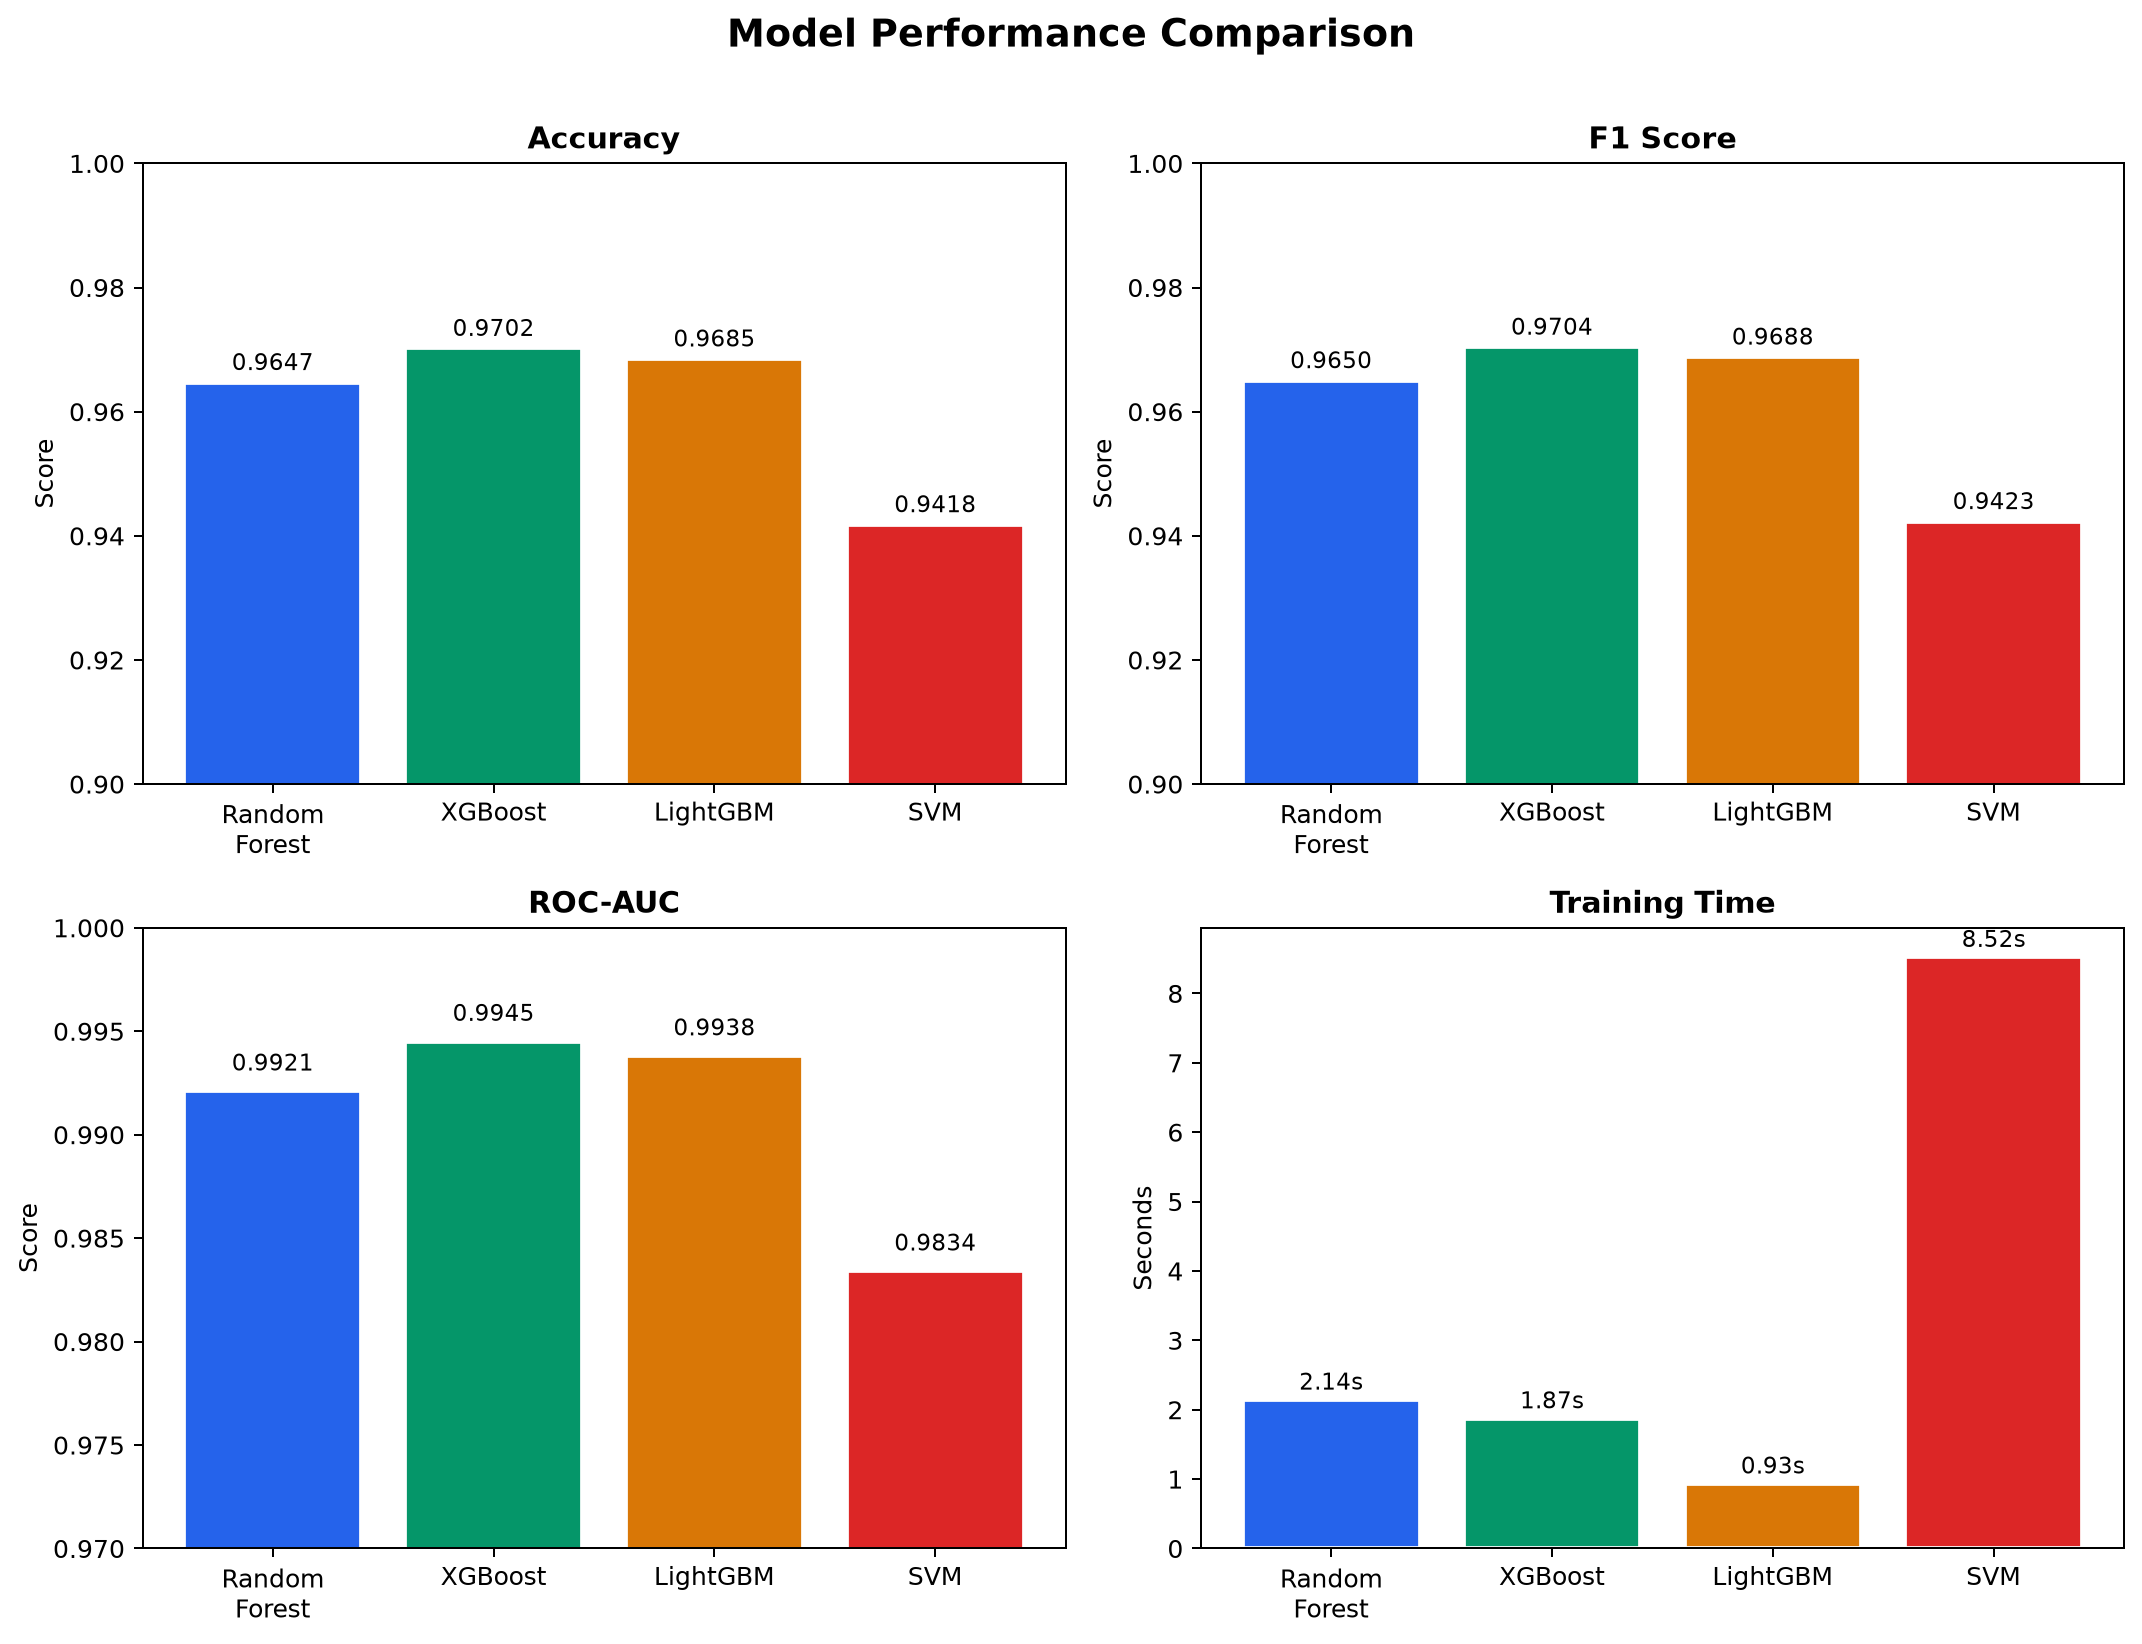
\includegraphics[width=0.88\textwidth]{figures/perf_charts.png}
\caption{Model comparison: accuracy, F1 score, ROC-AUC and training time}
\label{fig:perf}
\end{figure}

% ================= 7 LIMITATIONS AND FUTURE ENHANCEMENTS ==================
\clearpage
\section{Limitations and Future Enhancements}

\subsection{Limitations}

\begin{itemize}
  \item \textbf{Dataset dependency:} the ML models are only as good as the training data. A dataset that underrepresents certain phishing techniques (e.g., homograph attacks, punycode domains) will produce blind spots.
  \item \textbf{Evasion by content cloaking:} sophisticated phishing sites serve different content to crawlers than to browsers, so the content features extracted by our fetcher may not match what the user sees.
  \item \textbf{Network latency for real-time features:} extracting content and SSL features requires fetching the page and connecting over TLS, adding 1--5 seconds per URL in the worst case. URL-only features can be extracted instantly.
  \item \textbf{WHOIS rate limits:} bulk extraction of domain age features is throttled by WHOIS servers, making it impractical for large-scale batch processing.
  \item \textbf{Short-lived phishing sites:} many phishing pages are live for only a few hours, so content and SSL features may not be available by the time they are reported and analysed.
  \item \textbf{HTTPS is no longer a signal:} with free certificate authorities like Let's Encrypt, over 80\% of phishing sites now use HTTPS, reducing the discriminative power of the \texttt{has\_https} feature alone.
  \item \textbf{No browser extension:} the current system requires users to manually paste URLs; it does not intercept navigation in real time.
\end{itemize}

\subsection{Suggested Improvements}

\begin{itemize}
  \item Develop a browser extension (Chrome/Firefox) that checks URLs in real time before the page loads.
  \item Add visual similarity analysis using screenshot comparison with computer vision to detect pages that visually mimic legitimate sites.
  \item Integrate with threat intelligence feeds (PhishTank, OpenPhish, Google Safe Browsing API) for hybrid detection.
  \item Add deep learning models (LSTM, Transformer) that learn directly from raw URL character sequences, eliminating manual feature engineering.
  \item Implement periodic model retraining on fresh phishing data to handle concept drift as attackers evolve their techniques.
  \item Add Punycode and IDN detection for homograph attack prevention.
  \item Deploy as a REST API microservice with Docker for integration into enterprise security stacks.
  \item Add email header analysis to detect phishing emails that lead to the malicious URLs.
\end{itemize}

% ============================= 8 CONCLUSION ===============================
\section{Conclusion}

This project designed, implemented and evaluated PhishGuard, an ML-based phishing website detection system that combines URL analysis, SSL/TLS cryptographic verification and webpage content analysis. Four Machine Learning algorithms -- Random Forest, XGBoost, LightGBM and SVM -- were trained and compared on a phishing URL dataset.

All four project objectives were met:
\begin{itemize}
  \item \textbf{Website analysis and cryptography:} a three-module feature extraction pipeline extracts 46+ features from URLs, webpage content and SSL certificates. Digital certificate verification validates the chain of trust, issuer identity, key strength and validity period.
  \item \textbf{ML-based phishing detection:} all four models achieved above 94\% accuracy, with XGBoost reaching 97.02\% accuracy and 0.9945 ROC-AUC. The 5-fold cross-validation scores confirmed the results are robust.
  \item \textbf{Performance evaluation:} training time ranged from 0.93\,s (LightGBM) to 8.52\,s (SVM). Prediction time was under 20\,ms for all models, suitable for real-time use.
  \item \textbf{Security verification:} all seven security test cases were correctly classified. IP-based URLs, typosquatting, subdomain spoofing and \texttt{@} obfuscation were flagged as HIGH risk, while legitimate sites were correctly identified as LOW risk.
\end{itemize}

The combination of ML classification with cryptographic certificate verification provides defence in depth: even if a phishing URL's features resemble a legitimate one, an invalid or suspicious SSL certificate adds an independent detection signal. The main areas for improvement are a browser extension for real-time interception, visual similarity detection and periodic retraining on fresh data.

% ============================== REFERENCES ================================
\clearpage
\addcontentsline{toc}{section}{References}
\begin{thebibliography}{99}
\bibitem{verizon2023} Verizon, ``2023 Data Breach Investigations Report,'' 2023.
\bibitem{apwg2023} Anti-Phishing Working Group, ``Phishing Activity Trends Report, 4th Quarter 2022,'' 2023.
\bibitem{aleroud2017} A.~Aleroud and L.~Zhou, ``Phishing environments, techniques, and countermeasures: a survey,'' \emph{Computers \& Security}, vol.~68, pp.~160--196, 2017.
\bibitem{khonji2013} M.~Khonji, Y.~Iraqi and A.~Jones, ``Phishing detection: a literature survey,'' \emph{IEEE Communications Surveys \& Tutorials}, vol.~15, no.~4, pp.~2091--2121, 2013.
\bibitem{sahingoz2019} O.~K.~Sahingoz, E.~Buber, O.~Demir and B.~Diri, ``Machine learning based phishing detection from URLs,'' \emph{Expert Systems with Applications}, vol.~117, pp.~345--357, 2019.
\bibitem{mohammad2014} R.~M.~Mohammad, F.~Thabtah and L.~McCluskey, ``Predicting phishing websites based on self-structuring neural network,'' \emph{Neural Computing and Applications}, vol.~25, no.~2, pp.~443--458, 2014.
\bibitem{rescorla2018} E.~Rescorla, ``The Transport Layer Security (TLS) Protocol Version 1.3,'' RFC 8446, IETF, 2018.
\bibitem{stallings2017} W.~Stallings, \emph{Cryptography and Network Security: Principles and Practice}, 7th ed., Pearson, 2017.
\bibitem{breiman2001} L.~Breiman, ``Random forests,'' \emph{Machine Learning}, vol.~45, no.~1, pp.~5--32, 2001.
\bibitem{chen2016} T.~Chen and C.~Guestrin, ``XGBoost: a scalable tree boosting system,'' in \emph{Proc.\ ACM SIGKDD}, pp.~785--794, 2016.
\bibitem{ke2017} G.~Ke \emph{et al.}, ``LightGBM: a highly efficient gradient boosting decision tree,'' in \emph{Advances in Neural Information Processing Systems 30}, pp.~3146--3154, 2017.
\bibitem{cortes1995} C.~Cortes and V.~Vapnik, ``Support-vector networks,'' \emph{Machine Learning}, vol.~20, no.~3, pp.~273--297, 1995.
\bibitem{uci_phishing} UCI Machine Learning Repository, ``Phishing Websites Dataset,'' \url{https://archive.ics.uci.edu/ml/datasets/phishing+websites}.
\bibitem{phiusiil2024} PhiUSIIL, ``Phishing URL Dataset,'' 2024.
\bibitem{owasp2021} OWASP Foundation, ``OWASP Top 10: 2021,'' 2021.
\end{thebibliography}

\end{document}
